\documentclass[a4paper,papersize,10pt,twoside,uplatex,dvipdfmx]{jsarticle}
\usepackage[utf8]{inputenc}

%--余白の設定
\setlength{\topmargin}{10mm}
\addtolength{\topmargin}{-1in}
\setlength{\oddsidemargin}{10mm}
\addtolength{\oddsidemargin}{-1in}
\setlength{\evensidemargin}{10mm}
\addtolength{\evensidemargin}{-1in}
\setlength{\textwidth}{\paperwidth}
\addtolength{\textwidth}{-20mm}
\setlength{\textheight}{\paperheight}
\addtolength{\textheight}{-20mm}
\addtolength{\textheight}{-\headheight}
\addtolength{\textheight}{-\headsep}
\addtolength{\textheight}{-\footskip}
\setlength{\topskip}{0mm}

%ヘッダ・フッタの設定
\usepackage{fancyhdr}
\pagestyle{fancy}
\lhead[偶数ページ左側ヘッダ]{奇数ページ左側ヘッダ} 
\chead[偶数ページ中央ヘッダ]{奇数ページ中央ヘッダ}
\rhead[偶数ページ右側ヘッダ]{奇数ページ右側ヘッダ}
\lfoot[偶数ページ左側フッタ]{奇数ページ左側フッタ} 
\cfoot[偶数ページ中央フッタ]{奇数ページ中央フッタ} 
\rfoot[偶数ページ右側フッタ]{奇数ページ右側フッタ} 
\renewcommand{\headrulewidth}{3pt} %ヘッダの線の太さ 
\renewcommand{\footrulewidth}{3pt} %フッタの線の太さ

\title{テンプレート(とっても充実させた版)}
\author{author name}
\date{May 2019}

\usepackage{natbib}%\citep{},\citet{}命令を定義しているスタイルファイル
\usepackage{graphicx}%画像を張り込むのに必要

\begin{document}
\maketitle\thispagestyle{fancy}

\section{Introduction}
There is a theory which states that if ever anyone discovers exactly what the Universe is for and why it is here, it will instantly d\footnote{aiueitei}\footnote{skkdiss}isappear and be replaced by something even more {\Large bizarre and inexplicable}.
There is another theory which states that this has already happened.

\section{Introduction}
There is a theory which states that if ever anyone discovers exactly what the Universe is for and why it is here, it will instantly disappear and be replaced by something even more bizarre and inexplicable.
There is another theory which states that this has already happened.

\section{Introduction}
There is a theory which states that if ever anyone discovers exactly what the Universe is for and why it is here, it will instantly disappear and be replaced by something even more bizarre and inexplicable.
There is another theory which states that this has already happened.

\section{Introduction}
There is a theory which states that if ever anyone discovers exactly what the Universe is for and why it is here, it will instantly disappear and be replaced by something even more bizarre and inexplicable.
There is another theory which states that this has already happened.

\section{Introduction}
There is a theory which states that if ever anyone discovers exactly what the Universe is for and why it is here, it will instantly disappear and be replaced by something even more bizarre and inexplicable.
There is another theory which states that this has already happened.

\section{Introduction}
There is a theory which states that if ever anyone discovers exactly what the Universe is for and why it is here, it will instantly disappear and be replaced by something even more bizarre and inexplicable.
There is another theory which states that this has already happened.

\section{Introduction}
There is a theory which states that if ever anyone discovers exactly what the Universe is for and why it is here, it will instantly disappear and be replaced by something even more bizarre and inexplicable.
There is another theory which states that this has already happened.

\section{Introduction}
There is a theory which states that if ever anyone discovers exactly what the Universe is for and why it is here, it will instantly disappear and be replaced by something even more bizarre and inexplicable.
There is another theory which states that this has already happened.

\section{Introduction}
There is a theory which states that if ever anyone discovers exactly what the Universe is for and why it is here, it will instantly disappear and be replaced by something even more bizarre and inexplicable.
There is another theory which states that this has already happened.

\section{Introduction}
There is a theory which states that if ever anyone discovers exactly what the Universe is for and why it is here, it will instantly d\footnote{aiueitei}\footnote{skkdiss}isappear and be replaced by something even more bizarre and inexplicable.
There is another theory which states that this has already happened.

\section{Introduction}
There is a theory which states that if ever anyone discovers exactly what the Universe is for and why it is here, it will instantly disappear and be replaced by something even more bizarre and inexplicable.
There is another theory which states that this has already happened.

\section{Introduction}
There is a theory which states that if ever anyone discovers exactly what the Universe is for and why it is here, it will instantly d\footnote{aiueitei}\footnote{skkdiss}isappear and be replaced by something even more bizarre and inexplicable.
There is another theory which states that this has already happened.

\section{Introduction}
There is a theory which states that if ever anyone discovers exactly what the Universe is for and why it is here, it will instantly disappear and be replaced by something even more bizarre and inexplicable.
There is another theory which states that this has already happened.


\begin{figure}[h!]
\centering
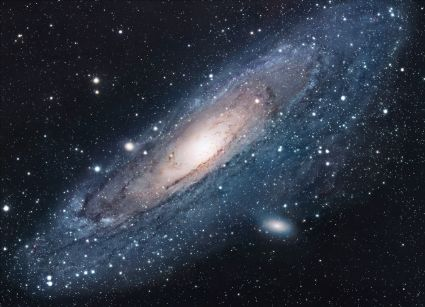
\includegraphics[scale=1.7]{universe}
\caption{The Universe}
\label{fig:universe}
\end{figure}

\section{Conclusion}
``I always thought something was fundamentally wrong with the universe'' \citep{adams1995hitchhiker}

\bibliographystyle{plain}
\bibliography{references}
\end{document}
